% Change these
\newcommand{\doctitle}{PID in State Space Form}
\date{\formatdate{13}{5}{2016}}

% Use to find math symbols:
%  http://detexify.kirelabs.org/classify.html

% "article" puts content on the first page, "report" does not
% letterpaper is 8.5"x11"
\documentclass[10pt,letterpaper]{article}
% Defaults
\usepackage[utf8]{inputenc}
\usepackage{amsmath}
\usepackage{amsfonts}
\usepackage{amssymb}
% Allow \href{http://url}{name}
\usepackage{hyperref}
\usepackage{xcolor}
\hypersetup{
    colorlinks=true,
    linkcolor={red!50!black},
    citecolor={blue!50!black},
    urlcolor={blue!80!black}
}
% Allow colored table rows
\usepackage{colortbl}
% Allow underline with \uline{text}
\usepackage[normalem]{ulem}
% Allow monospace with \begin{lstlisting}
\usepackage{listings}
\usepackage{textcomp}
\lstset{basicstyle=\ttfamily,
%escapeinside={||}, % Allow Latex inside escaped
mathescape=false, % Allow $$ to be displayed
columns=fullflexible, % Don't add extra spaces
upquote=true, % Use normal quotes
showspaces=false,
showstringspaces=false,
prebreak = \raisebox{0ex}[0ex][0ex]{\ensuremath{\hookleftarrow}} % nod idea
}
% Syntax highlighted code. Notes:
%  - requires installing "minted" from AUR
%  - requires adding "-shell-escape" to the pdflatex command
\usepackage{minted}
% Allow single, double, etc. spacing
\usepackage{setspace}
% Allow setting a date with \formatdate{day}{month}{year}
\usepackage[USenglish]{babel}
\selectlanguage{USenglish}
\usepackage{datetime}
% Make " do the correct left/right quotes
\usepackage [autostyle, english=american]{csquotes}
\MakeOuterQuote{"}
% Margins since the default are huge
\usepackage[top=1in, bottom=1in, left=1in, right=1in]{geometry}
% Shrink the section font size
%\usepackage{sectsty}
%\sectionfont{\fontsize{10}{10}\selectfont}
% Allow embedding images from this path
\usepackage{graphicx}
\graphicspath{ {./} }
% Allow subfigures
\usepackage{subfig}
% Allow Roman numeral lists
\usepackage{enumerate}
% Even and odd numbering
\usepackage{enumitem}
\newlist{oddenumerate}{enumerate}{1}
\setlist[oddenumerate]{start=0,label=\theoddenumeratei.}
\newlist{evenenumerate}{enumerate}{1}
\setlist[evenenumerate]{start=0,label=\theevenenumeratei.}
\makeatletter
\renewcommand\theoddenumeratei{\@arabic{\numexpr2*\value{oddenumeratei}+1}}
\renewcommand\theevenenumeratei{\@arabic{\numexpr2*\value{evenenumeratei}+2}}
\makeatother
% Don't indent paragraphs
\usepackage{parskip}
\setlength{\parindent}{0pt}
% Page header
\usepackage{fancyhdr}
\pagestyle{fancy}
% Allow using the "independent" math symbol
\newcommand\independent{\protect\mathpalette{\protect\independenT}{\perp}}
\def\independenT#1#2{\mathrel{\rlap{$#1#2$}\mkern2mu{#1#2}}}
% Displayed on first page, escape # character
\title{\doctitle}
\author{Garrett Wilson}
% Redefine author and title so they can be used after \maketitle
\makeatletter
\let\mauthor\@author
\let\mtitle\@title
\makeatother
% Header left, center, and right at the top of all but the first page
\lhead{\mauthor}
\rhead{\doctitle}
%\chead{\homework}

\begin{document}
\maketitle
\subsection*{Why?}
It should be possible to write your PID controller in state space form. This is an attempt at doing that. This could be used to compare your state space controller with your PID controller in simulation.

\subsection*{The Math}
A PID controller normally looks like the following:

\[u(t) = k_p e(t) + k_i \int_{0}^{t} e(\tau) d\tau + k_d \dot{e}(t) \]

We want to try rewriting this in state space form. Our state space form looks like:

\begin{equation} \label{eq:state}
\dot{x} = ax+bu
\end{equation}
\begin{equation} \label{eq:output}
y = cx
\end{equation}

Let us define our error to be the difference between our output and our set point (the desired output):

\[ e \equiv y - s = cx - s \]

Now let's look at the three different components of the feedback term $u$ that will in the end be summed together in our PID controller. For the proportional term:

\[ u = -k_p e \]

For the integral term, let's define a new variable $z$ whose derivative is the error $e$ so that $z$ is the integral of the error:

\[ \dot{z} \equiv e \]
\[ u = -k_i z \]

Finally, for the derivative,

\[ u = -k_d \dot{y} \]

Note that we're using $\dot{y}$ rather than $\dot{e}$, but these will be equivalent except for when the set point $s$ changes. It is preferable to use $\dot{y}$ since the derivative is defined even if $s$ changes instantaneously. This is one of the approaches Wikipedia lists to get around step changes in $s$, another one being to never have a step change but gradually move between the old and new values.

We will use our model of the system to calculate $\dot{y} = c \dot{x}$:

\[ \dot{y} = c \dot{x} = c (ax + bu) \]
\[ \implies u = -k_d c (ax + bu) \]

Notice that we have a $u$ on both the left and right sides of the equation. Solving for $u$:

\[ \implies u + k_d c b u = -k_d c a x \]
\[ \implies ( 1 + k_d c b ) u = -k_d c a x \]
\[ \implies u = - k_d ( 1 + k_d c b )^{-1} c a x \]

And let's define $K_g$ to make this easier to read:

\[ K_g \equiv ( 1 + k_d c b )^{-1} \]
\[ \implies u = - k_d K_g c a x \]

Now let's sum all of these P, I, and D components of the feedback input $u$:

\[ u = -k_p e -k_i z - k_d K_g c a x \]

And define $y_p$, $y_i$, and $y_d$ to be:

\begin{equation} \label{eq:y_p}
y_p \equiv e = \dot{z} = cx - s
\end{equation}
\begin{equation} \label{eq:y_i}
y_i \equiv z
\end{equation}
\begin{equation} \label{eq:y_d}
y_d \equiv K_g c a x
\end{equation}

Then, rewriting $u$ in terms of these new variables:

\begin{equation} \label{eq:u}
u = -k_p y_p -k_i y_i - k_d y_d
\end{equation}

We want to write all of this in state space. In addition to our original $x$ state (or vector of states), let's add an additional state for $z$ since the we need $z$ in our PID controller for the integral term. For the state equation $\dot{X} = AX + BU$, using $\dot{z} = cx - s$ and equation \ref{eq:state}:

\begin{equation} \label{eq:complete_state}
\begin{bmatrix}
    \dot{x} \\
    \dot{z} \\
\end{bmatrix} =
\begin{bmatrix}
	a & 0 \\
	c & 0 \\
\end{bmatrix}
\begin{bmatrix}
	x \\
	z \\
\end{bmatrix} + 
\begin{bmatrix}
	b & 0 \\
	0 & -1 \\
\end{bmatrix}
\begin{bmatrix}
	u \\
	s \\
\end{bmatrix}
\end{equation}

For the output $Y = CX + DU$, we want to not only get the system output $y$ but also the three terms we'll be using in our PID control law. Using equations \ref{eq:output}, \ref{eq:y_p}, \ref{eq:y_i}, \ref{eq:y_d}:

\begin{equation} \label{eq:complete_output}
\begin{bmatrix}
	y \\
	y_p \\
	y_i \\
	y_d \\
\end{bmatrix} =
\begin{bmatrix}
	c & 0 \\
	c & 0 \\
	0 & 1 \\
	K_g c a & 0 \\
\end{bmatrix}
\begin{bmatrix}
	x \\
	z \\
\end{bmatrix} + 
\begin{bmatrix}
	0 & 0 \\
	0 & -1 \\
	0 & 0 \\
	0 & 0 \\
\end{bmatrix}
\begin{bmatrix}
	u \\
	s \\
\end{bmatrix}
\end{equation}

Finally, we can write the control law:

\[ u = -K Y \]
\[
K \equiv
\begin{bmatrix}
	0 & k_p & k_i & k_d
\end{bmatrix}
\]

It would be nice if we could get something we could run through $lsim$ nicely. If we plug the control law back into our state space equations, rewriting it without the $u$ input, using equations \ref{eq:u} and \ref{eq:complete_state}:

\[
\begin{bmatrix}
    \dot{x} \\
    \dot{z} \\
\end{bmatrix} =
\begin{bmatrix}
	a & 0 \\
	c & 0 \\
\end{bmatrix}
\begin{bmatrix}
	x \\
	z \\
\end{bmatrix} + 
\begin{bmatrix}
	b & 0 \\
	0 & -1 \\
\end{bmatrix}
\begin{bmatrix}
	-k_p y_p -k_i y_i - k_d y_d \\
	s \\
\end{bmatrix}
\]

Then, plugging in \ref{eq:y_p}, \ref{eq:y_i}, and \ref{eq:y_d}:

\[
\begin{bmatrix}
    \dot{x} \\
    \dot{z} \\
\end{bmatrix} =
\begin{bmatrix}
	a & 0 \\
	c & 0 \\
\end{bmatrix}
\begin{bmatrix}
	x \\
	z \\
\end{bmatrix} + 
\begin{bmatrix}
	b & 0 \\
	0 & -1 \\
\end{bmatrix}
\begin{bmatrix}
	-k_p (cx - s) -k_i z - k_d K_g c a x \\
	s \\
\end{bmatrix}
\]

With a little bit more algebra, we get:

\begin{equation} \label{eq:final_state}
\begin{bmatrix}
    \dot{x} \\
    \dot{z} \\
\end{bmatrix} =
\begin{bmatrix}
	a - b (k_p c + k_d K_g c a) & -b k_i \\
	c & 0 \\
\end{bmatrix}
\begin{bmatrix}
	x \\
	z \\
\end{bmatrix} + 
\begin{bmatrix}
	b k_p \\
	-1 \\
\end{bmatrix} s
\end{equation}

For the output, let's just look at the original $y$ as in equation \ref{eq:output}:

\begin{equation} \label{eq:final_output}
y = \begin{bmatrix}
	c & 0 \\
\end{bmatrix}
\begin{bmatrix}
	x \\
	z \\
\end{bmatrix}
\end{equation}

\subsection*{Example}
Let's try out a PID controller on a second-order system of a mass, spring, and a force applied to the right on the mass.

\begin{center}
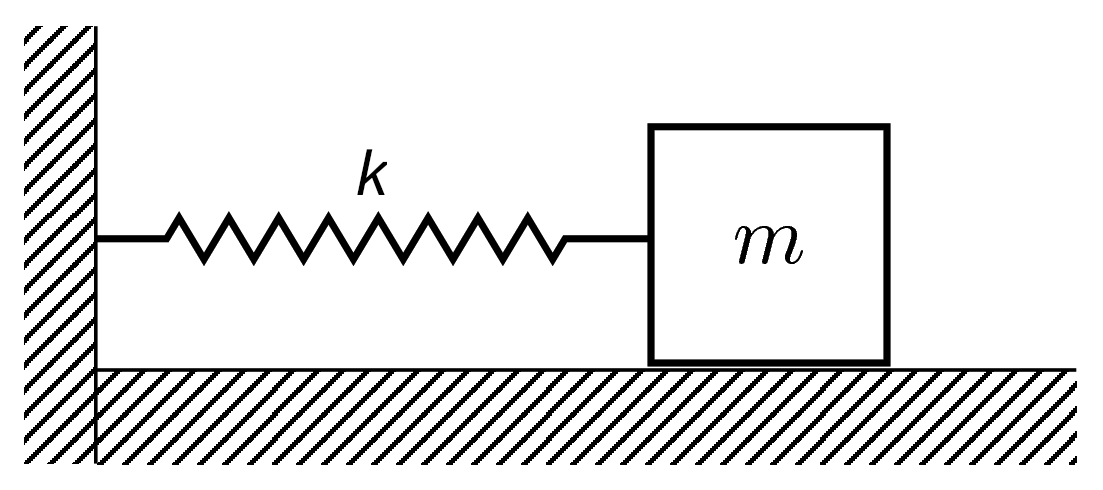
\includegraphics[scale=0.2]{spring-mass}
\end{center}

Writing the state space equations $\dot{w} = Aw + Bu$ and $y = Cw = Du$:

\[
\begin{bmatrix}
	\dot{x} \\
	\ddot{x} \\
\end{bmatrix} =
\begin{bmatrix}
	0 & 1 \\
	-k/m & 0 \\
\end{bmatrix}
\begin{bmatrix}
	x \\
	\dot{x} \\
\end{bmatrix} +
\begin{bmatrix}
	0 \\
	1/m \\
\end{bmatrix} F
\]

\[
y =
\begin{bmatrix}
	x \\
	\dot{x} \\
\end{bmatrix}
\]

So,

\[
A = \begin{bmatrix}
	0 & 1 \\
	-k/m & 0 \\
\end{bmatrix}, \qquad
B = \begin{bmatrix}
	0 \\
	1/m \\
\end{bmatrix}, \qquad
C = I_2 = \begin{bmatrix}
	1 & 0 \\
	0 & 1 \\
\end{bmatrix}, \qquad
D = 0
\]

When converting our PID controller to state space, we'll have to make the $C$ matrix only have a single output (it may be possible to do more, but so far I have only made it work with a single output):

\[
C = \begin{bmatrix}
	1 & 0 \\
\end{bmatrix}
\]

Below is the open-loop response and the response with an LQR, PID, and the PID in state space form controllers.

\begin{center}
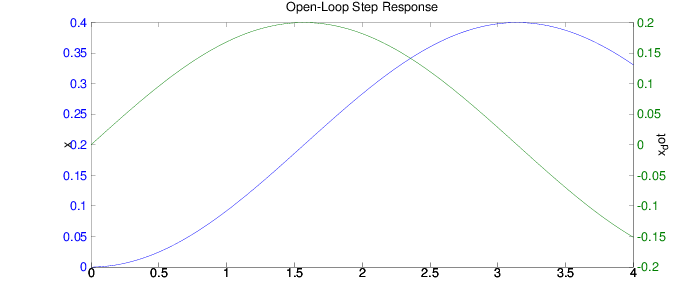
\includegraphics[scale=0.6]{image-ol}
\end{center}

\begin{center}
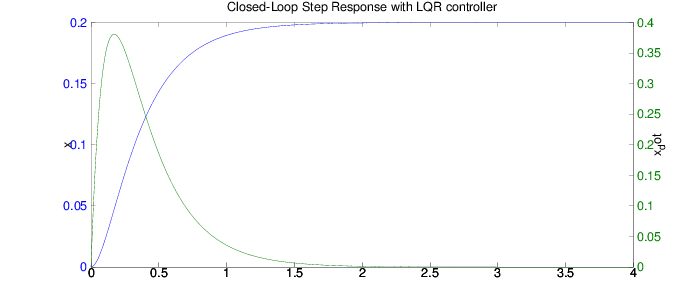
\includegraphics[scale=0.6]{image-lqr}
\end{center}

\begin{center}
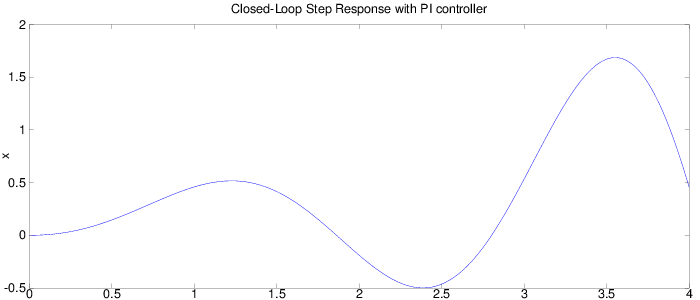
\includegraphics[scale=0.6]{image-pi}
\end{center}

\begin{center}
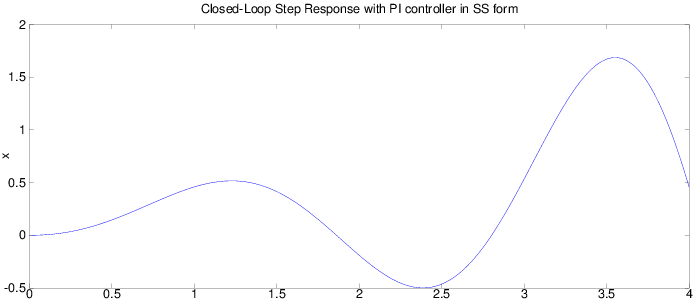
\includegraphics[scale=0.6]{image-pi-ss}
\end{center}

\begin{center}
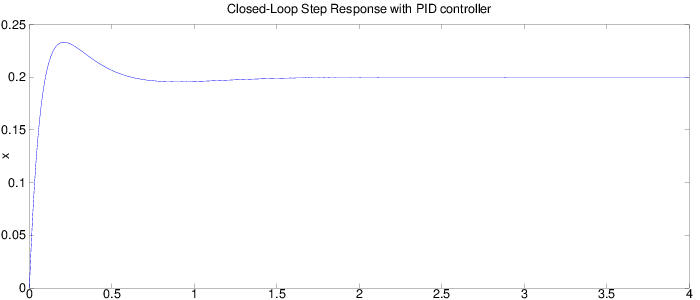
\includegraphics[scale=0.6]{image-pid}
\end{center}

\begin{center}
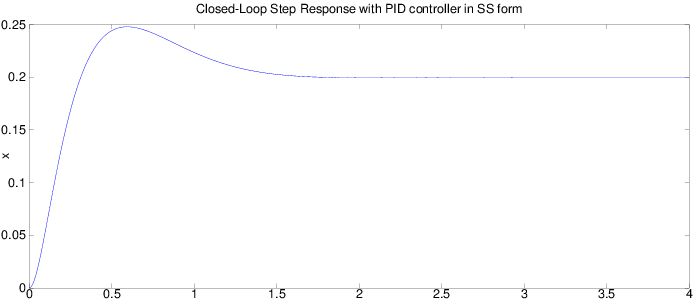
\includegraphics[scale=0.6]{image-pid-ss}
\end{center}

You'll notice the PID in state space form response is different from the PID response but the PI in state space is exactly the same as the PI response. They will look exactly the same if we set $k_d = 0$. However, if $k_d \neq 0$, then it might different because in the straight PID controller, the derivative is not calculated based on the system model. More work needs to be done to explore how we can get these to match when using a derivative term.

\subsection*{Octave Code for Example}
\begin{minted}[mathescape,
               linenos,
               numbersep=5pt,
               frame=lines,
               framesep=2mm]{matlab}
pkg load control;

doPlot = true;

% Plot both x and x_dot
function plotResponse(sys, plotTitle)
figure;
t = 0:0.01:4;
r = 0.2*ones(size(t));
[y,t,x]=lsim(sys,r,t);
[AX,H1,H2] = plotyy(t,y(:,1),t,y(:,2),'plot');
set(get(AX(1),'Ylabel'),'String','x');
set(get(AX(2),'Ylabel'),'String','x_dot');
title(plotTitle)
end

% Plot only x
function plotResponseSingle(sys, plotTitle)
figure;
t = 0:0.01:4;
r = 0.2*ones(size(t));
[y,t,x]=lsim(sys,r,t);
plot(t,y,'-b');
ylabel('x');
title(plotTitle)
end

% State space for simple second-order spring-mass equation
k = 1;
m = 1;

A = [0 1; -k/m 0];
B = [0; 1/m];
C = eye(2);
D = 0;

states = {'x' 'x_dot'};
inputs = {'F'};
outputs = {'x'; 'x_dot'};
sys_ss = ss(A,B,C,D,
    'statename',states,
    'inputname',inputs,
    'outputname',outputs);
if doPlot
    plotResponse(sys_ss, 'Open-Loop Step Response');
    print -dpng -S"700,300" -F"Helvetia:6" image-ol.png
end

% Controller using LQR
Q = C'*C;
Q(1,1) = 10;
R = 0.01;
K = lqr(A,B,Q,R);

% Correct position error
Cn = [1 0];
sys_nbar = ss(A,B,Cn,0);
Nbar = rscale(sys_nbar,K);

Ac = [(A-B*K)];
Bc = [B*Nbar];
Cc = [C];
Dc = [D];

sys_cl = ss(Ac,Bc,Cc,Dc,
    'statename',states,
    'inputname',inputs,
    'outputname',outputs);
if doPlot
    plotResponse(sys_cl,
        'Closed-Loop Step Response with LQR controller');
    print -dpng -S"700,300" -F"Helvetia:6" image-lqr.png
end

% Use a PID controller
Kp = 100;
Ki = 200;
Kd = 20;

% We need to have SISO, so redefine C to only give us x out
C_siso = [1 0];
outputs_siso = {'x'};
sys_ss_siso = ss(A,B,C_siso,D,
    'statename',states,
    'inputname',inputs,
    'outputname',outputs_siso);
sys_tf = tf(sys_ss_siso);

pid_controller = pid(Kp,Ki,Kd);
sys_cl_pid = feedback(pid_controller*sys_tf,1);
if doPlot
    plotResponseSingle(sys_cl_pid,
        'Closed-Loop Step Response with PID controller');
    print -dpng -S"700,300" -F"Helvetia:6" image-pid.png
end

% Now let's use our new PID in SS form controller
%
% Note: We're using C_siso since with a PID controller you only have one
% output.
Kg = inv(1 + Kd*C_siso*B);

% Check to verify that the issue isn't in removing u from the state space
% equations. It's not. This basically is the same as when using lsim.
%
% To check transfer function in sage:
%    factor(matrix([1,0,0])*~(matrix([[s,0,0],[0,s,0],[0,0,s]])-
%      matrix([[0,1,0],[-101,-20,-200],[1,0,0]]))*matrix([[0],[100],[-1]]))
%
% Compare:
%    feedback(pid(Kp,Ki,Kd)*sys_tf,1)
%    tf(sys_ss_pid)
if doPlot && false
    % The open-loop A, B, C, and D
    Apid_ol = [A zeros(size(A,1),1); C_siso zeros(1,1)];
    Bpid_ol = [B zeros(size(B,1),1); 0 -1];
    Cpid_ol = [C_siso 0; C_siso 0; zeros(1,size(C,2)) 1; Kg*C_siso*A 0];
    Dpid_ol = [0 0; 0 -1; 0 0; 0 0];

    % Discretize to have our own lsim-like simulation
    f = 100;
    T = 1/f;
    sys_d = c2d(ss(Apid_ol,Bpid_ol,Cpid_ol,Dpid_ol), T, 'zoh');

    N = 4*f;
    state = zeros(size(C_siso,2)+1, 2);
    output = zeros(N, size(Dpid_ol,1));

    % Constant set point
    s = 0.2;
    input = zeros(N,2);

    for i = 2:N
        input(i,:) = [-[0 Kp Ki Kd]*output(i-1,:)'; s]';
        state(:,1) = sys_d.a*state(:,2) + sys_d.b*input(i,:)';
        output(i,:) = sys_d.c*state(:,2) + sys_d.d*input(i,:)';
        state(:,2) = state(:,1);
    end

    t = 0:T:(size(output,1)-1)/f;
    figure;
    plot(t,output(:,1));
    ylabel('x');
    title('PID in SS - without lsim');
end

Apid = [A-B*(Kp*C_siso+Kd*Kg*C_siso*A) -B*Ki; C_siso 0];
Bpid = [B*Kp; -1];
Cpid = [C_siso 0];
Dpid = 0;

states_pid = {'x' 'x_dot' 'z'};
inputs_pid = {'s'};
sys_ss_pid = ss(Apid,Bpid,Cpid,Dpid,
    'statename',states_pid,
    'inputname',inputs_pid,
    'outputname',outputs_siso);
if doPlot
    plotResponseSingle(sys_ss_pid,
        'Closed-Loop Step Response with PID controller in SS form');
    print -dpng -S"700,300" -F"Helvetia:6" image-pid-ss.png
end

% These should be the same
%feedback(pid(Kp,Ki,Kd)*sys_tf,1)
%tf(sys_ss_pid)

% Just use a PI controller, which does look the same
Kp = 5;
Ki = 10;
Kd = 0;

pid_controller = pid(Kp,Ki,Kd);
sys_cl_pid = feedback(pid_controller*sys_tf,1);
if doPlot
    plotResponseSingle(sys_cl_pid,
        'Closed-Loop Step Response with PI controller');
    print -dpng -S"700,300" -F"Helvetia:6" image-pi.png
end

Kg = inv(1 + Kd*C_siso*B);
Api = [A-B*(Kp*C_siso+Kd*Kg*C_siso*A) -B*Ki; C_siso 0];
Bpi = [B*Kp; -1];
Cpi = [C_siso 0];
Dpi = 0;

sys_ss_pi = ss(Api,Bpi,Cpi,Dpi,
    'statename',states_pid,
    'inputname',inputs_pid,
    'outputname',outputs_siso);
if doPlot
    plotResponseSingle(sys_ss_pi,
        'Closed-Loop Step Response with PI controller in SS form');
    print -dpng -S"700,300" -F"Helvetia:6" image-pi-ss.png
end
\end{minted}

\subsection*{Sources}
A significant portion of the math comes from here, but I used $\dot{z} = cx - s$ rather than $\dot{z} = b_e y_p$ (at Frohne's suggestion) since it made the end result look cleaner. I continued on to find the $A$, $B$, $C$, and $D$ matrices if the only input we have is the set point $s$ rather than both $u$ and $s$ so we can simulate this with $lsim$. And, I also did not set $u = v + s$ but only $u = v$ to make this more like a normal PID controller.

\url{http://home.earthlink.net/~ltrammell/tech/pidvslin.htm}

Describes three approaches to deal with instantaneous step changes in the set point, one of which is by using $\dot{y}$ rather than $\dot{e}$:

\url{https://en.wikipedia.org/wiki/PID_controller#Setpoint_step_change}

Image of the spring-mass system:

\url{https://minireference.com/_media/physics/mass_spring-highres.png}

\end{document}
